% !TeX spellcheck = it_IT
\newpage
\section{Design pattern}
La progettazione non è solo un processo creativo. Il progettista può infatti seguire una serie di regole pratiche, appunto i design patterns, che descrivono il cuore della soluzione ad un problema frequente in modo che questa possa essere riutilizzata tante volte.\\

Nel software in particolare i pattern (soluzioni create in passato) vengono utilizzati per avere una maggiore \textbf{produttività} e rendere i progetti più \textbf{flessibili}.\\

\subsection{Gang of Four}
\subsubsection{Classificazione}
Nell'ambito della \textbf{progettazione di dettaglio}, \textbf{GoF} i pattern sono classificati in base al loro scopo e divisi in tre categorie:
\begin{itemize}
	\item \textbf{Creazionali}: riguardano la creazione di oggetti
	\begin{itemize}
		\item \textit{Abstract Factory}
		\item \textit{Builder}
		\item \textit{Factory Method}
		\item \textit{Prototype}
		\item \textit{Singleton}
	\end{itemize}
	\item \textbf{Strutturali}: riguardano la composizione di classi ed oggetti
	\begin{itemize}
		\item \textit{Adapter}
		\item \textit{Bridge}
		\item \textit{Composite}
		\item \textit{Decorator}
		\item \textit{Façade}
		\item \textit{Flyweight}
		\item \textit{Proxy}
	\end{itemize}
	\item \textbf{Comportamentali}: riguardano le interazioni tra classi ed oggetti e la suddivisione delle loro responsabilità
	\begin{itemize}
		\item \textit{Chain of responsibility}
		\item \textit{Command}
		\item \textit{Interpreter}
		\item \textit{Iterator}
		\item \textit{Mediator}
		\item \textit{Memento}
		\item \textit{Observer}
		\item \textit{State}
		\item \textit{Strategy}
		\item \textit{Template}
		\item \textit{Visitor}
	\end{itemize}
\end{itemize}

\newpage
\subsubsection{Template}
Un buon template per un pattern secondo GoF è il seguente:
\begin{table}[!h]
	\centering
	\begin{tabular}{|c|c|}
		\hline
		\textbf{Pattern name and classification} & Un nome breve e conciso per un pattern ed il suo tipo \\
		\hline
		\textbf{Intent} & Una breve frase su cosa fa il pattern \\
		\hline
		\textbf{Also known as} & Altri nomi \\
		\hline
		\textbf{Motivation} & Uno scenario che mostri perché è utile \\
		\hline
		\textbf{Applicability} & Situazioni dove può essere usato \\
		\hline
		\textbf{Structure} & Rappresentazione grafica \\
		\hline
		\textbf{Participants} & Le classi e gli oggetti che lo compongono\\
		\hline
		\textbf{Collaborations} & Come i partecipanti rispettano le loro responsabilità \\
		\hline
		\textbf{Consequences} & Pro e contro \\
		\hline
		\textbf{Implementation} & Suggerimenti e tecniche per l'implementazione \\
		\hline
		\textbf{Sample code} & Frammenti di codice per una semplice implementazione \\
		\hline
		\textbf{Known users} & Esempi in sistemi reali \\
		\hline
		\textbf{Related patterns} & Altri pattern strettamente correlati \\
		\hline
	\end{tabular}
\end{table}

\subsubsection{Notazione}
GoF utilizza come notazione la \textbf{Object Modeling Technique}.
\begin{center}
	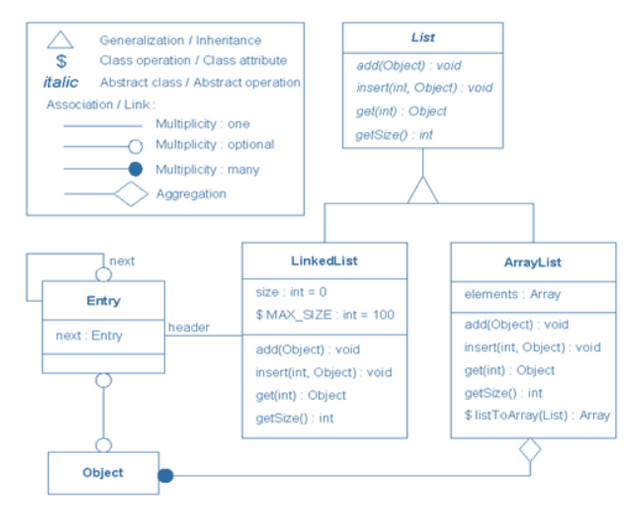
\includegraphics[scale=.5]{gof}
\end{center}

\newpage
\subsection{Strategy}
Lo strategy design pattern prevede di definire una famiglia di algoritmi, incapsularli separatamente e renderli intercambiabili. Questo permette ad essi di cambiare indipendentemente dai clienti che li usano.\\
Un programma potrebbe dover fornire più \textbf{varianti} di un algoritmo: le variazioni vengono incapsulate in classi separate mentre il metodo per l'accesso ad esse rimane uniforme.\\
Lo strategy design pattern si compone di tre partecipanti:
\begin{itemize}
	\item \textbf{Strategy}: definisce un'interfaccia comune per gli algoritmi
	\item \textbf{ConcreteStrategy}: ogni strategia concreta implementa un algoritmo
	\item \textbf{Context}: contiene un riferimento ad un oggetto \textit{strategy} e può definire un'interfaccia che le consente di accedere ai dati di interesse invece di doverli passare come argomenti
\end{itemize}

\begin{example}[MyArray]
	La classe \textit{MyArray} rappresenta un vettore di numeri. Uno dei suoi metodi lo stampa in due possibili formati che potrebbero però cambiare in futuro:
	\begin{itemize}
		\item \textit{MathFormat}, e.g. $\{12,-7,3,\ldots\}$
		\item \textit{StandardFormat}, e.g. ar[0]=12, ar[1]=-7, ar[2]=3,...
	\end{itemize}
	Usiamo lo strategy design pattern per isolare l'algoritmo di formattazione in modo che possa variare indipendentemente dal resto della classe.
	\begin{center}
		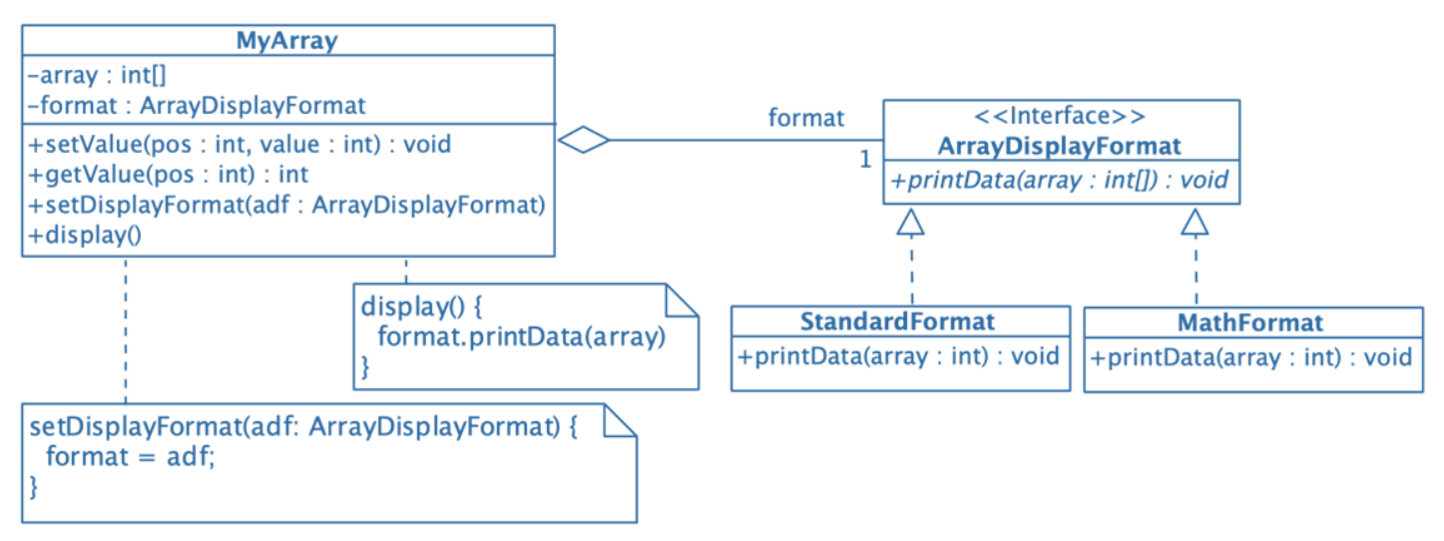
\includegraphics[scale=.3]{myarray}
	\end{center}
	La \textit{strategy} è \textit{ArrayDisplayFormat}, le \textit{ConcreteStrategy} sono \textit{StandardFormat} e \textit{MathFormat} e il \textit{Context} è \textit{MyArray}.
\end{example}

\subsubsection{Conclusioni}
Lo strategy pattern è utile nei seguenti casi:
\begin{itemize}
	\item Più classi correlate differiscono solo nel \textbf{comportamento}
	\item Servono più \textbf{varianti} diverse di un algoritmo
	\item Un algoritmo usa dei dati che i clienti non conoscono
	\item Evitare di esporre strutture dati complesse e algorithm-specific
\end{itemize}

\begin{note}
	Quando una classe definisce molti comportamenti che appaiono come alternative in costrutti condizionali, può essere utile trasformare i branch in classi ottenute con lo strategy pattern.
\end{note}

Il \textbf{costo} dello strategy pattern è di incrementare il numero di oggetti presenti in un'implementazione e la necessità di garantire che le implementazioni diverse rispettino la stessa interfaccia.

\begin{observation}[Dati diversi]
	Può capitare che strategie diverse usino dati diversi e che quindi in certe \textit{ConcreteStrategy} non tutti i dati vengano utilizzati. Per evitare l'inizializzazione di questi ultimi, si deve fare un \textbf{coupling} maggiore tra \textit{ConcreteStrategy} e \textit{Context}, dove le prime devono chiedere al secondo solo i dati necessari.
\end{observation}
\subsection{State}
Lo state design pattern è un \textbf{behavioural pattern}, ovvero che consente ad un oggetto di alterare il suo comportamento quando cambia lo stato interno. Si compone di tre partecipanti:
\begin{itemize}
	\item \textbf{Context}: definisce l'interfaccia di interesse per i client e mantiene un'istanza di \textit{ConcreteState} che definisce lo stato corrente
	\item \textbf{State}: incapsula il comportamento associato ad un particolare stato del \textit{Context}. Può anche essere una classe concreta con un'implementazione predefinita.
	\item \textbf{Concrete state}: sono sottoclassi dello stato che implementano il comportamento associato allo \textit{State} che rappresentano.
\end{itemize}
Vediamo i passaggi per implementare lo state pattern:
\begin{enumerate}
	\item Identificare o creare una classe (\textbf{Context}) che funga da macchina a stati dal punto di vista del cliente
	\item Creare una classe \textbf{State} che replichi i metodi dell'interfaccia della macchina a stati: ogni metodo richiederà un parametro aggiuntivo (un'istanza della classe di \textit{Context})
	\item Creare una \textbf{sottoclasse} di \textit{State} per ogni stato del dominio, ognuna delle quali sovrascrive solo i metodi che cambiano
	\item La classe di \textit{Context} mantiene lo \textbf{stato corrente}, che è un oggetto della classe di \textit{State}
	\item Le richieste dei client sono delegate dalla classe di \textit{Context} allo stato corrente, passando ad esse anche l'oggetto di \textit{Context}
	\item I metodi della classe \textit{State} modificano lo stato corrente
\end{enumerate}

\begin{example}[TCP]
	Un esempio è l'implementazione del protocollo TCP, che invia risposte diverse a seconda dello stato della connessione.
	\begin{center}
		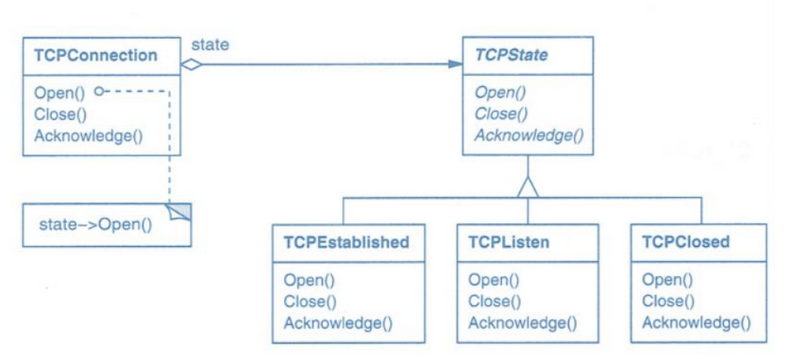
\includegraphics[scale=.4]{tcp}
	\end{center}
\end{example}

\subsubsection{Conclusioni}
Lo state pattern è utile nei seguenti casi:
\begin{itemize}
	\item Il \textbf{comportamento} di un oggetto dipende dal suo stato
	\item Le operazioni hanno \textbf{dichiarazioni condizionali complesse}, dove la scelta dipende dallo stato
\end{itemize}

\begin{observation}
	Il comportamento è suddiviso tra i possibili stati e ognuno è memorizzato in una classe.
\end{observation}
\begin{observation}
	Lo stato corrente è memorizzato in un'unica posizione e le transizioni di stato sono esplicite.
\end{observation}
\begin{observation}
	La classe \textit{State} può implementare parte del comportamento se è in comune o di default. Inoltre i suoi oggetti possono essere condivisi quando non hanno variabili di istanza.
\end{observation}

\subsection{Factory}
Le factory sono dei pattern di tipo \textbf{creazionale}: astraggono il processo di instanziazione degli oggetti nascondendo l'effettiva creazione e rendendo il sistema indipendente da ciò.\\
Una classe \textit{factory} ha il solo compito di creare e restituire istanze di altre classi.

\begin{observation}[New]
	Il comando \textit{new} viola il principio \textit{code to an interface} in quanto assegniamo ad una variabile un oggetto ottenuto da una classe concreta. Questa dipende da ogni classe riferita al suo interno e deve essere aggiornata e ricompilata se cambiano le classi riferite, violando i principi \textit{open-closed} e \textit{information hiding}.
\end{observation}

\subsubsection{Simple factory}
Detto anche ConcreteFactory, non appartiene alla Gang of Four ed è una semplificazione molto diffusa di \textit{Abstract Factory}. Consiste nel delegare ad un oggetto \textbf{factory} la creazione separandola dalle altre funzionalità.
\begin{center}
	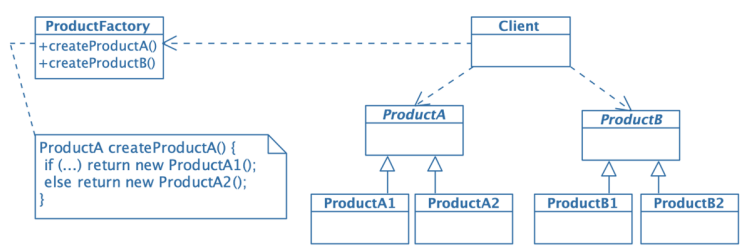
\includegraphics[scale=.5]{simplefactory}
\end{center}

\subsubsection{Factory method}
Il factory method delega alle sottoclassi la decisione di quali classi istanziare. Si compone di quattro partecipanti:
\begin{itemize}
	\item \textbf{Creator} (astratto o concreto): dichiara il \textbf{factory method} che viene usato da altri metodi. Questo, se crea tipi diversi di prodotti, deve avere un parametro.
	\item \textbf{ConcreteCreator}: sovrascrive il \textit{factory method} per restituire un istanza del \textit{ConcreteProduct}
	\item \textbf{ConcreteProduct}: implementa l'interfaccia di \textit{Product}
	\item \textbf{Product}: definisce l'interfaccia per il tipo di oggetti che sono creati dal \textit{factory method}
\end{itemize}
\begin{center}
	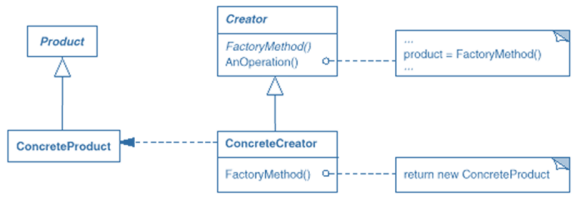
\includegraphics[scale=.6]{factorymethod}
\end{center}

Il factory method pattern permette di disaccoppiare una classe dalle classi degli oggetti che crea e utilizza e delega alle sottoclassi la specifica degli oggetti da creare. Rende il codice più \textbf{flessibile} e \textbf{riusabile} e implementa il principio di \textit{code to an interface} (la classe si basa sull'interfaccia di \textit{Product} e può funzionare con qualunque \textit{ConcreteProduct} che la supporti).\\

Lo \textbf{svantaggio} principale è la necessità di estendere la classe \textit{Creator} solo per istanziare un particolare \textit{ConcreteProduct}.

\subsubsection{Abstract factory}
L'abstract factory delega ad altre classi la decisione di quali classi istanziare. Definisce un'interfaccia per creare famiglie di oggetti correlati e dipendenti fra loro senza specificare le classi concrete.\\
A differenza del \textit{factory method}, l'abstract delega ad altri oggetti l'istanziazione tramite la \textbf{composizione}. Questi altri oggetti spesso usano il \textit{factory method}.
\begin{center}
	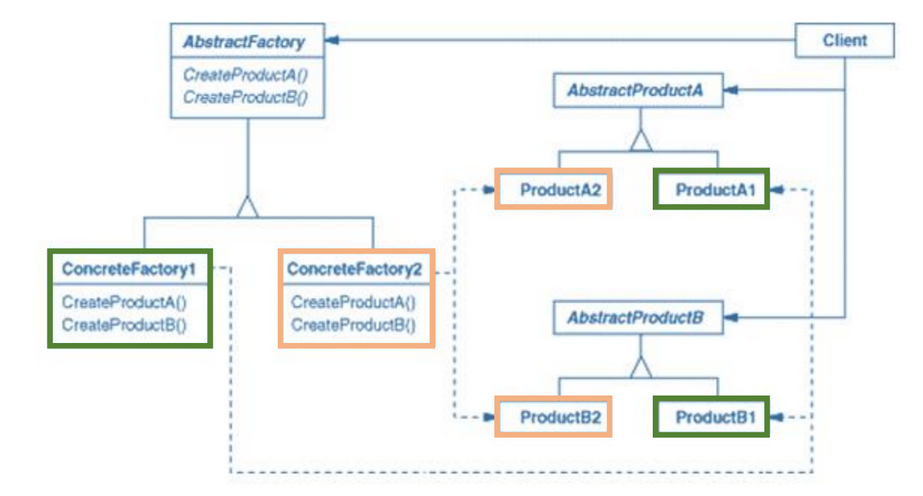
\includegraphics[scale=.3]{abstractfactory}
\end{center}

\subsubsection{Pure fabrication}
Si tratta di un pattern \textbf{GRASP} che assegna responsabilità fortemente correlate ad una \textbf{classe artificiale} che non rappresenta niente nel dominio del problema (è introdotta solo per convenienza). Implementa il \textbf{behavioural decomposition} con l'obiettivo di supportare \textit{high coesion}, \textit{low coupling} e \textit{riuso}.

\subsection{Singleton}
Il singleton pattern garantisce che una classe abbia \textbf{una sola istanza} fornendo un punto di accesso globale ad essa. 
\begin{note}
	Nonostante la necessità di avere oggetti unici sia abbastanza comune, in quanto spesso gran parte degli oggetti in un'applicazione hanno un'unica responsabilità assegnata, le classi singleton sono rare.
\end{note}
\noindent Per costruirlo:
\begin{enumerate}
	\item Si rende privato il costruttore della classe
	\item Si aggiunge un oggetto statico privato che conterrà l'unica istanza disponibile
	\item Si rende l'unica istanza disponibile accessibile solo tramite un metodo statico
\end{enumerate}

\begin{wrapfigure}[5]{r}{4cm}
	\vspace{-.5cm}
	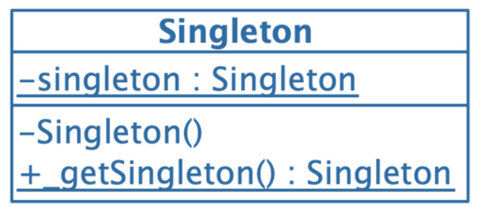
\includegraphics[width=4cm]{singleton}
\end{wrapfigure}
\subsubsection{Inizializzazione lazy} A volte non si potrebbero avere \textbf{sufficienti informazioni} per l'istanziazione del singleton statico oppure potrebbe essere molto \textbf{resource intensive}. In questo caso è meglio aspettare per eseguire l'inizializzazione.

\subsubsection{Multithread} Thread diversi potrebbero inizializzare più istanze del singleton quasi simultaneamente. Ci sono tre possibili soluzioni:
\begin{itemize}
	\item \textbf{Inizializzazione eager} invece di quella \textit{lazy}, spreca risorse
	\item \textbf{Sincronizzazione} del metodo \textit{getInstance}, dichiarandolo come \textit{synchronized}, riduce le performance
	\item \textbf{Double-checked locking}: una variabile volatile garantisce che ogni thread acceda all'ultimo valore assegnatole e solo un thread alla volta può eseguire un blocco di codice synchronized.
\end{itemize}

\subsubsection{Sottoclassi}
Nel caso in cui una classe singleton venga estesa, per garantire che l'unica istanza sia istanza di una sottoclasse, facciamo in modo che ognuna di esse fornisca un metodo statico \textit{getIstance}. In questo modo i costruttori delle sottoclassi possono essere privati e quello del singleton sarà \textbf{protected}.